\section{Hyperparameter overview}

Building the different models for the procedure illustrated in figure \ref{fig:model_training_concept} requires to make a number of choices.
In this section, these components are introduced.

\subsection{Network types\label{sec:network_types}}

Three different \acrlong{cnn} architectures were tested for this project:
\begin{description}
    \item[the VGG16 network: ] classic, added some upscore layers.
    \item[The RESNET50 network:] skip connections
    \item[The U-Net network: ] good performance for some biological problems
\end{description}

All of these networks function based on the \textit{encoder - decoder} principle.
\todo{add more insights on the principle}

\begin{SCfigure}[][htb]
    \centering
    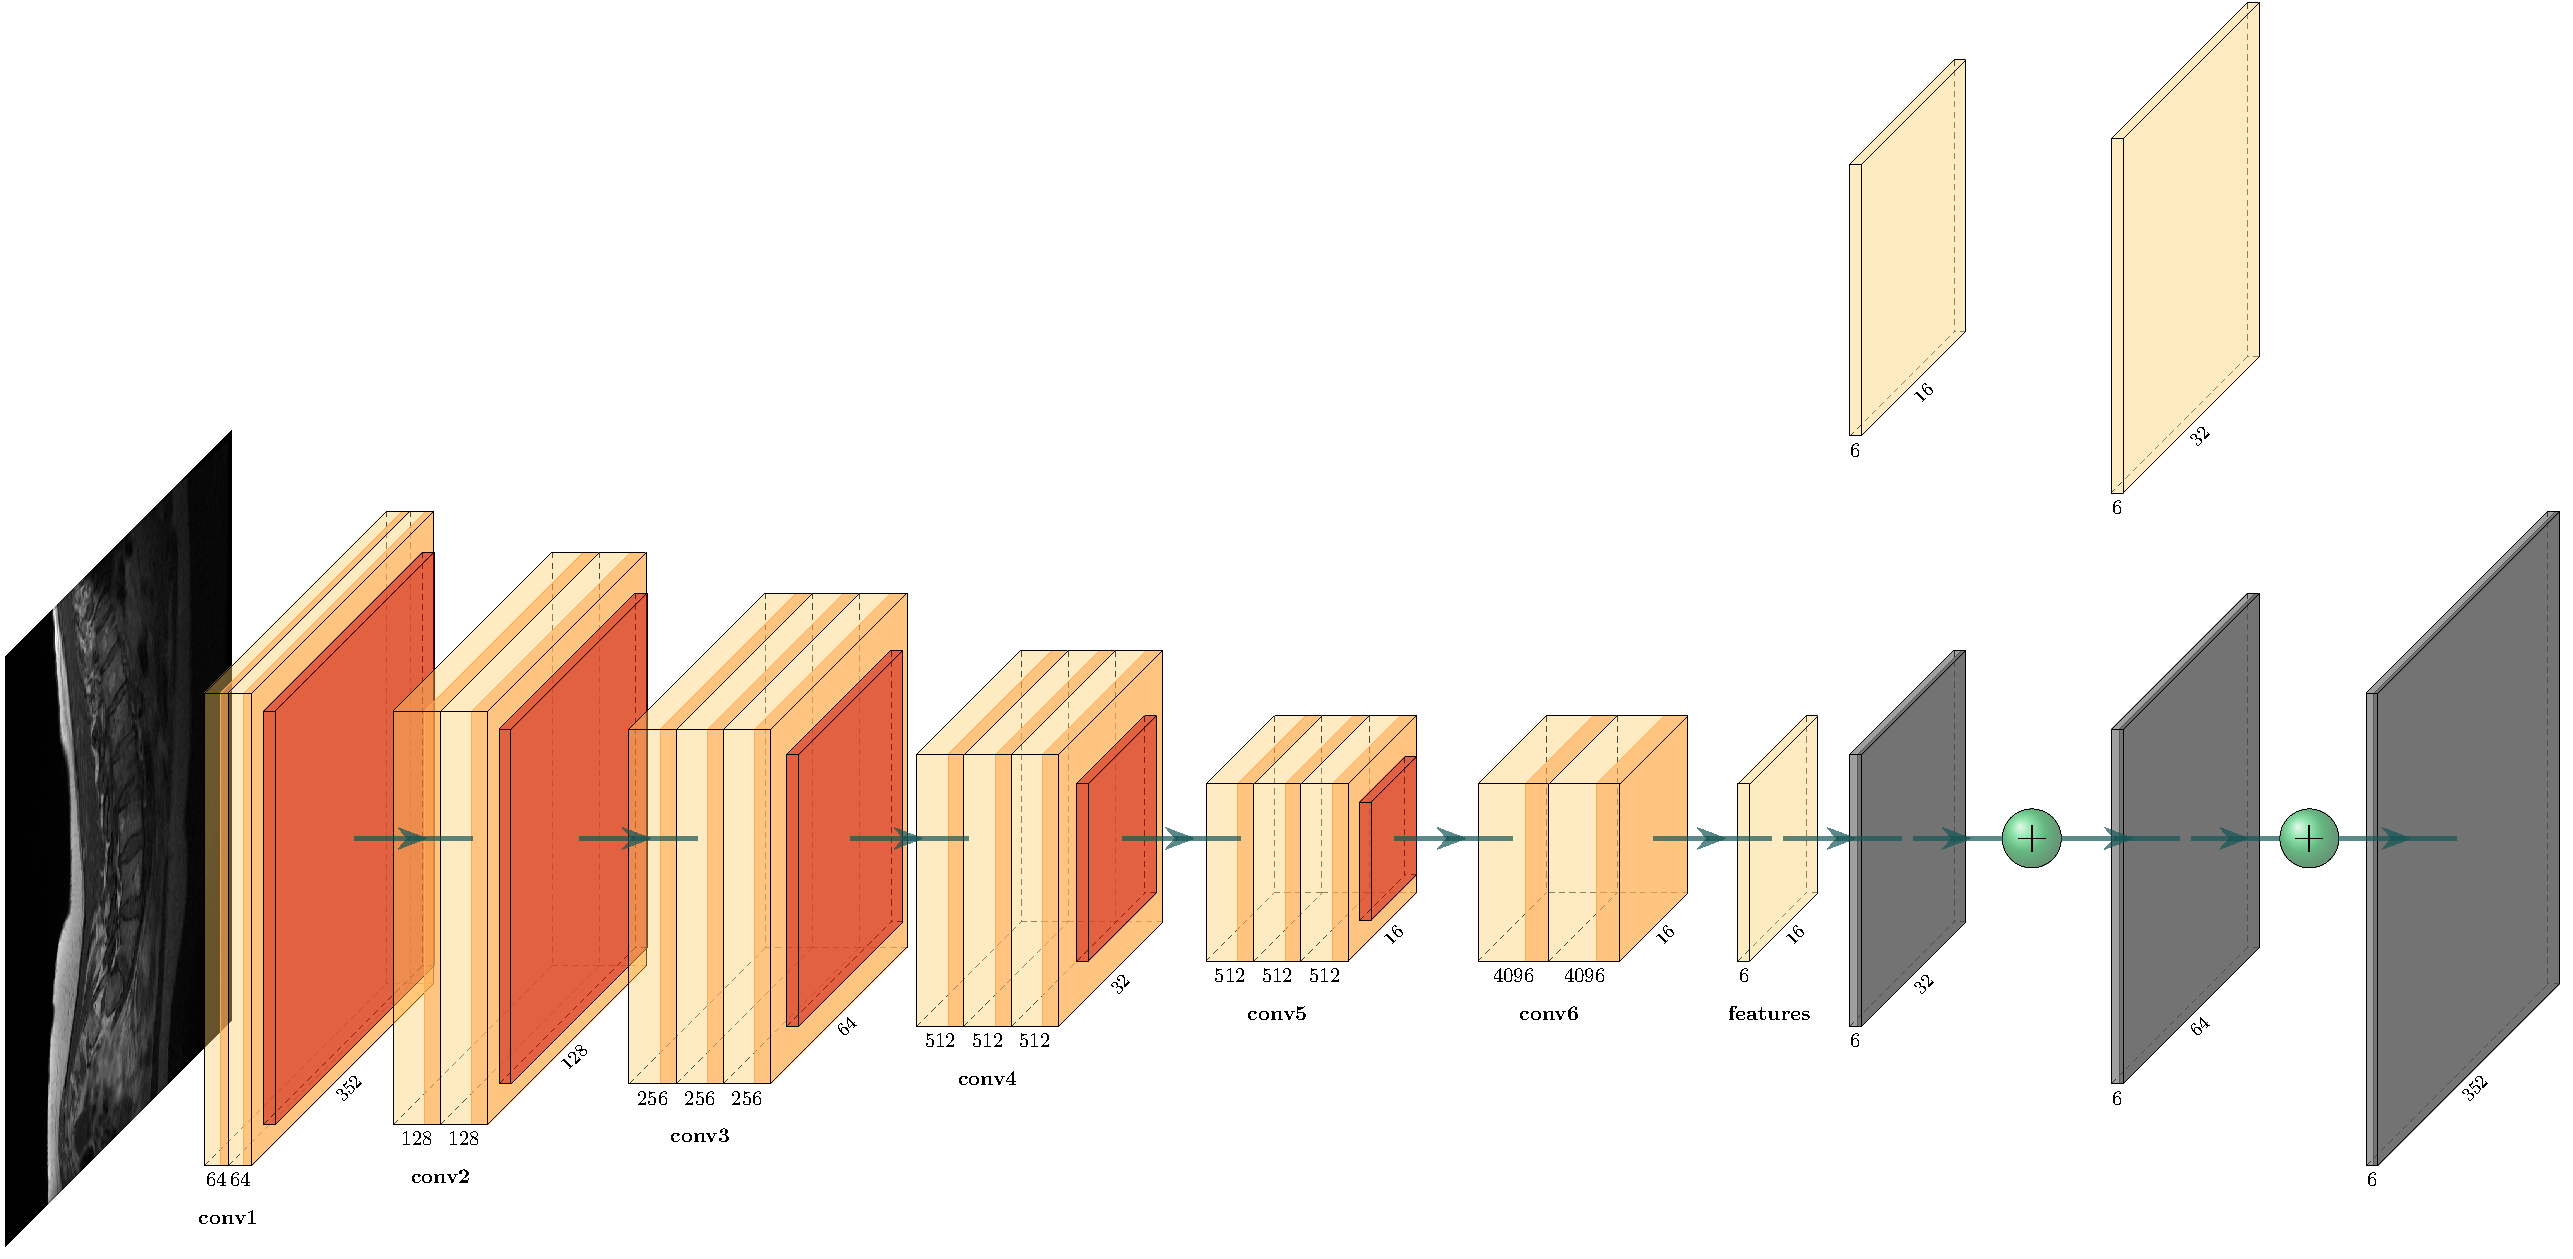
\includegraphics[width=.95\textwidth]{vgg16_upscore.pdf}
    \caption{VGG16 based network}
\end{SCfigure}

\begin{SCfigure}[][htb]
    \centering
    \includegraphics[width=.95\textwidth]{unet.pdf}
    \caption{Unet based network}
\end{SCfigure}

\subsection{2D+ approach and \textit{context slices}\label{section:twoDplus}}

As discussed in section \ref{sec:network_types}, all used networks have a 3 channel\footnote{The networks were originally designed for \textit{RGB}-images with a red, a green and a blue channel.}, 
352$\times$352 pixel input. 
The input images for the network only have 1 channel component. 
The other two channels were used to pass \textit{context} information to the network in the form of the neighboring slices of the slice under investigation.
This combines an essentially 2D approach with a third dimensional element in the form of the extra information of the parallel slices. Thus, this is called the $2D+$ approach.


The hyperparameter to be set $k$ is the index offset for the context slices.
When evaluating slice with index $n$ the slices with indices $\left[n-k; n+k\right]$ are passed as context slices
\footnote{For the edge cases ($n<k$ or $n+k>$ image dimension) when these slices do not exist, slice $n$ is passed as context slice.}.


Several values for $k$ are tested. When $k=0$, no extra slices are taken. The same slice is just entered in all 3 network channels. When $k=1$, the indices directly next to the investigated slices are taken.
Due to the isotropic resampling (see section \ref{sec:resampling}), these slices are physically at 1 mm distance of the center slice. When $k=5$, the slices at $5 mm$ distance from the center slice are used.